\section{\textbf{Dissertation Proposal: Monte Carlo and Portable Performance}}

This section considers Monte Carlo transport applications in the context of portable performance as a proposed dissertation research plan.
%
Efforts in Ray Tracing using the EAVL/VTK-m framework showed significant success~\cite{larsen2015ray} and provide workloads that are similar to those used in Monte Carlo transport problems.
%
However, Monte Carlo transport offers a unique set of challenges and interesting lessons when evaluating portable performance possibilities that are not covered through similar algorithms.
%
These challenges include: complex/random data access patterns in many nested steps, many nested levels of divergence, and complex output tally systems.
%
In addition, the idea of portable performance is popular with many different groups, who are putting forward possible designs and library options.
%
Each of these designs or abstraction layers --- listed in Section~\ref{sec:whatispp} --- has its own pluses and minuses, as well as requiring different amounts of effort in order to make it function within already existing codes.
%

%
The following sections discuss in detail the research plan for completing a dissertation.
%
First is a discussion of recently completed work with a Monte Carlo research application, ALPSMC~\cite{alpsmc1}~\cite{alpsmc2}, where the algorithmic question of event-based versus history-based algorithms choice was evaluated.
%
In addition, the effects that different parallel paradigms have on performance as well as the ease of code conversion were studied in this work.
%
Following is a discussion of future work directions and a path to completing a dissertation.

\subsection{\textbf{Work to date: ALPSMC}}

ALPSMC~\cite{brantley2011benchmark} is a Monte Carlo test code that models neutron transport in a one dimensional planar geometry, through a binary stochastic medium.
%
It is originally a serial C++ application that follows an all particle history-based approach.
%
This history-based algorithm is shown in Algorithm~\ref{alg:history-based}.
%

\begin{algorithm}
\DontPrintSemicolon
\caption{History-based Monte Carlo algorithm}
\label{alg:history-based}
\ForEach{particle history}
{ 
    generate particle from boundary condition or source\;
    \While{particle not escaped or absorbed}
    {
       sample distance to collision in material\;
       sample distance to material interface\;
       compute distance to cell boundary\;
       select minimum distance, move particle, and perform event\;
       \If{particle escaped spatial domain}
       {
          update leakage tally\;
          end particle history\;
       }
       \If{particle absorbed}
       {
          update absorption tally\;
          end particle history\;
       }
    }
}
\end{algorithm}
%

%
The original work was to convert this algorithm into an event-based approach.
%
The event-based algorithm performs data parallel operations across all of the particles that are in the same event, as well as a series of data parallel steps required to do proper bookkeeping to get the particles for each event.
%
The event-based algorithm is defined in Algorithm~\ref{alg:eventbased}.
%
The operations required to launch the event kernels are defined as follows and correspond to lines 6 and 7 of Algorithm~\ref{alg:eventbased}~\cite{alpsmc1}.
%
\begin{itemize}
\item{[Step 1:]} thrust::transform --- Fill out a stencil map of 1's and 0's of all particles doing event E (where each particle whose next event is E will get a 1 in the stencil map at its index location)
\item{[Step 2:]} thrust::reduce --- Count the number of elements labeled 1 in the stencil (determines the number of particles that will perform event E)
\item{[Step 3:]} Check if the number of elements is greater than 0 (check if any particles are performing event E)
\item{[Step 4:]} thrust::exclusive\_scan --- generate indices for index mapping from stencil map (indices for each particle performing event E)
\item{[Step 5:]} Allocate a new map of appropriate size (map to hold indices for all particles performing event E)
\item{[Step 6:]} Scatter indexes from scan into new index map (reduces the exclusive\_scan generated indices into the map that holds only enough for particles performing event E)
\item{[Step 7:]} Use new index map in permutation\_iterator loops over all particles (combining the index map with the permutation iterator allows loops over all particles to operate only on the particles selected in the index map)
\end{itemize}
%

\begin{algorithm}
\DontPrintSemicolon
\caption{Event-based Monte Carlo algorithm}
\label{alg:eventbased}
\ForEach{batch of particle histories (fits in memory constraint)}
{ 
    generate all particles in batch from boundary condition or source\;
    determine next event for all particles (collision, material interface crossing, cell boundary crossing)\;
    \While{particles remaining in batch}
    {
       \ForEach{event E in (collision, material interface crossing, cell boundary crossing)}
       {
          identify all particles whose next event is E\;
          perform event E for identified particles and determine next event for these particles\;
       }
       \If{particle escaped spatial domain}
       {
          update leakage tally\;
       }
       \If{particle absorbed}
       {
          update absorption tally\;
       }
       delete particles absorbed or leaked\;
    }
}
\end{algorithm}

Thrust was chosen as the platform for implementing the data parallel operations, though many of the options discussed would have worked for this.
%
The key design choice was that each operation can be done using data parallel primitives.
%
This study also used a direct CUDA implementation that launched kernels for the main events and used Thrust for data management for comparison.

The performance results from the initial implementation~\cite{alpsmc1} were varied.
The best CUDA version had speedups ranging from around 6X to 12X, while the Thrust CUDA version only achieved a range of around 2X to 2.5X.
%
Additionally the Thrust OpenMP version reached at most 2.2X with 16 threads.
%
The optimized implementation discovered a few areas for improvement and achieved fairly significant improvements for all cases.
%
Table~\ref{tab:ALPSspeedup} shows the summary of ALPSMC speedup results after the optimization pass~\cite{alpsmc2}.
%

\begin{table}
\caption { Maximum speedups for each approach when compared to the original history-based serial method } \label{tab:ALPSspeedup} 
\begin{center}
\begin{tabular}{ |c|c|}
\hline
Method & Speedup\\
\hline
CUDA Event SOA & 31.32\\
\hline
CUDA History & 52.78\\
\hline
Thrust Event CUDA SOA & 54.62\\
\hline
Thrust Event OpenMP SOA & 5.54\\
\hline
\end{tabular}
\end{center}
\end{table}

Through this experience we have demonstrated a few important points.
%
First we demonstrated excellent performance in both algorithms, achieving \textasciitilde50x performance for both history and event-based algorithms.
%
Scudiero~\cite{tonyScudiero} showed similar success with a history-based approach and explained that the primary concern of Monte Carlo transport on GPUs is actually memory latency and that divergence does not significantly impact results in a memory latency bound problem.
%
Additionally, these examples showed that using the data parallel design and an abstraction layer -- in this case Thrust -- can perform just as well as when programmed in native CUDA under some circumstances. 
%
Lastly, while the GPU performance is high the CPU performance is still lacking.
%
Figure~\ref{fig:OMPScale} shows that the OpenMP version scales well but it has a much higher overhead than the original serial version.

\begin{figure}
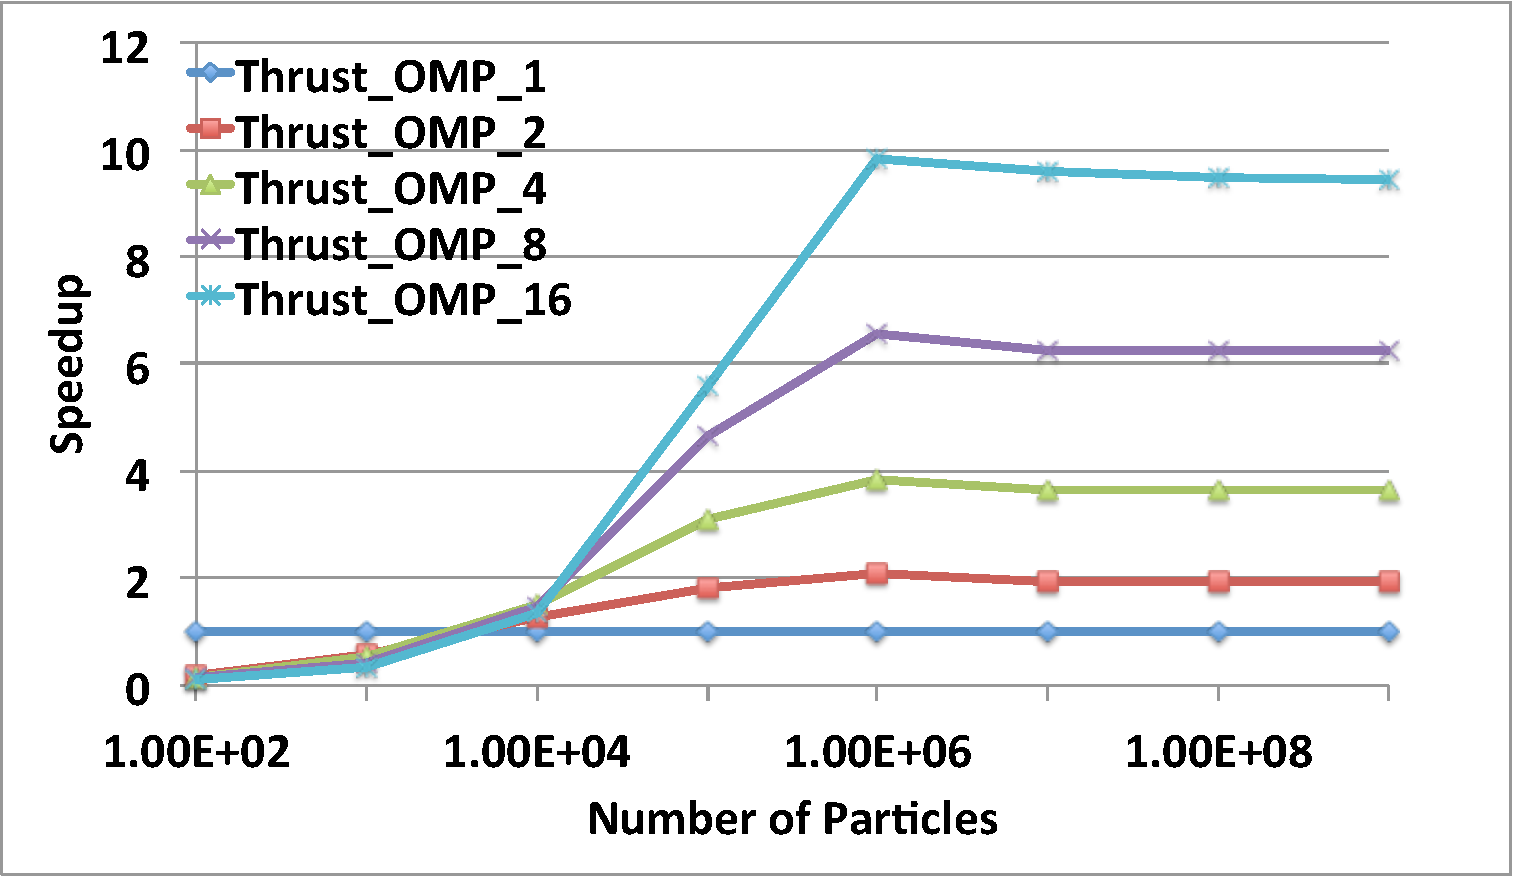
\includegraphics[width=0.49\textwidth]{thrustOMPSpeedup.pdf}
\caption{Speedups versus number of particles for the event-based Thrust CPU method with 1, 2, 4, 8, 16 OpenMP threads compared to the Thrust CPU method serially.~\cite{alpsmc2}}
\label{fig:OMPScale}
\end{figure}

All of these considerations lay a foundation for future study.
%
ALPSMC is a small test code that functions like a mini app to a larger application.
%
Since ALPSMC does simplify many of the complex parts of the Monte Carlo transport problem the actual speedups may not accurately reflect the final performance possibilities of a more fully featured Monte Carlo transport code.
%

\subsection{\textbf{Future Work}}

This survey has addressed the history of Monte Carlo transport applications and research with respect to parallelism.
%
In this survey we have seen that there has been a major revival of computational studies with every new generation of supercomputing platform.
%
Monte Carlo transport applications have only one significant gap in knowledge where groups have just recently started adding supporting research.
%
That area is the case of a fully featured Monte Carlo application on GPUs and scalable to high numbers of GPUs, which is an increasingly prevalent design for leading-edge supercomputers.

Previous thesis work lays a starting foundation to build upon, but does not begin to provide a full solution for other groups to follow.
%
One significant hurdle in the Monte Carlo transport world is the necessary redesign for GPU hardware.
%
It is important for groups to not need to rewrite their entire applications, which can consist of hundreds of thousands of lines of code.
%
Codes like MCNP~\cite{goorley2012initial}~\cite{padovani2012mcnpx}, Mercury~\cite{brantley2013recent}, and even OpenMC~\cite{romano2015openmc}
will all be faced with many decisions on how to progress into the future of computing.

The OpenMC group has started looking into this problem through the use of mini applications, RSBench~\cite{tramm2014performance} and XSBench~\cite{tramm2014xsbench}. 
%
This approach allows groups to focus on the specific areas that are important to them and optimize an easier to manipulate application before attempting any changes on a full scale production application.
%
One of the major focuses of this work has been in the area of continuous energy cross section searches, since for a large number of their problems that functionality took \textasciitilde85\% of their workload.

As with many other groups the Mercury group at LLNL has also begun work on a mini application.
%
This application is different to RSBench and XSBench in multiple ways but most significantly it uses the multi group energy cross sections and emphasizes  many of the key areas of the Mercury production application.
%
This application will provide a beginning point for the redesign of the Mercury Monte Carlo code and allow for a rich research environment for upcoming years.
%

I propose to work under the Mercury group on the Quicksilver mini application, in order to develop a scalable GPU version of the code in a way that can translate to direct modifications of the production application.
%
I will further explore the event versus history-based dilemma under the Quicksilver application in order to understand the potential performance when compared to the much larger necissary redesign.
%
I also plan on exploring the potential for a hybrid event/history algorithm that might utilize the advantages of both when possible.
%
I also plan on using the data parallel primitive design scheme as well as some layer of abstraction to make my research portable to multiple architecture platforms.
%
Additionally, there are a number of optimizations, data structures, and smaller research problems to tackle along the path of development.
%
Finally, I plan on summarizing the results of my research through large scale testing on the Trinity MIC platform, as well as the not yet released Sierra NVIDIA Volta platform.

The goal of this research will be to provide a concrete path forward for the Mercury team as well as provide a mini application that scales well on both of the competing top architectures at once.
%
This path involved many as of yet unanswered questions and a clear path of research for providing new an unique research to this field.




